% Plantilla simple para tareas de la Licenciatura en Física
% Fer Flores - Universidad de Guadalajara - Noviembre 2023

%%%%%%%%%%%%%%%%%%%%%%%%%%%%%%%%%%%%%%%%%%-PREÁMBULO-%%%%%%%%%%%%%%%%%%%%%%%%%%%%%%%%%%%%%%%%%%

% Paqueterías

\documentclass{assignment}
\usepackage[pdftex]{graphicx} % FIGURAS
\usepackage{xcolor}
\definecolor{LightGray}{gray}{0.95}
\usepackage{fancyvrb, minted} % CÓDIGO
\usepackage[letterpaper, margin = 2.5cm]{geometry} % TAMAÑO DE PÁGINA Y MÁRGENES
\usepackage[T1]{fontenc} % Importante para acentos automáticos y símbolos de escritura
% \usepackage[spanish, mexico]{babel} % Importante para Español
\usepackage{amsmath, amsfonts, amssymb} % Ecuaciones, caracteres y símbolos especiales
\usepackage{hyperref, url}  % Links y Hyperlinks en el documento
\usepackage{fancyhdr}
\usepackage{enumitem}
\usepackage{listings}
\usepackage{amsmath}
\usepackage{graphicx}
%-----------------------------------------ETIQUETAS--------------------------------------------

\student{Revin Dsilva \\ rd3387}                             % NOMBRE
\semester{Spring 2024}                                % SEMESTRE (202X A/B)
\date{\today}                                   % Fecha (Modifica a DD/MM/AAAA)

\courselabel{CS6923}          % CLAVE Y MATERIA
\exercisesheet{Introduction to Machine Learning}{Written Homework 1}     % NÚMERO Y TÍTULO DE LA TAREA

\school{Tandon School of Engineering}          % CARERA (Física, la mejor carrera)
\university{New York University}         % LA PODEROSÍSIMA

%%%%%%%%%%%%%%%%%%%%%%%%%%%%%%%%%%%%%%%%%%-DOCUMENTO-%%%%%%%%%%%%%%%%%%%%%%%%%%%%%%%%%%%%%%%%%%%%

\begin{document}

%-----------------------------------------------------------------------------------------------
\begin{problem}

\section{Problem 1: Practicing Minimizing a Loss Function}

\noindent Consider a linear model of the form:

\begin{equation}\label{eq:Equation}
     f_\beta(x) = \beta x,
\end{equation}
which is the same as the linear model we saw in class, but with the intercept forced to zero. Such models are used when we want to force the predicted value $f_\beta(x) = 0$ when $x = 0$. For example, if we are modeling $y$ = output power of a motor vs. $x$ = the input power, we would expect $x$ = 0 $\implies$  $y$ = 0.
\begin{enumerate}[label=(\alph*)]
\item Given data $(x_1,y_1 ),.....,(x_n,y_n )$, write the equation for a loss function which measures prediction accuracy using the sum-of-squared distances between the predicted values and target values.

\item Derive an expression for the $\beta$ that minimizes this loss function. Do you get the same expression that
we got for $\beta_1$
in the full linear model?

\end{enumerate}


\subsubsection*{Solution 1 (a)}

\noindent In class, we discussed the linear model of the form: 
     $f_\beta(x) = \beta_0 + \beta_1 x$, 
in which we had the intercept $\beta_0$. 
In the linear model given in the question we have the intercept to be 0. Thus the loss function for the linear model $f_\beta(x) = \beta x$ becomes 
\begin{equation}\label{eq:Equation}
     L(\beta) = \sum_{i=1}^{n} (y_i - f_\beta(x_i))^2
\end{equation}
\begin{equation}\label{eq:Equation}
     L(\beta) = \sum_{i=1}^{n} (y_i -  \beta x_i)^2
\end{equation}

\subsubsection*{Solution 1 (b)}

\noindent To derive the expression for $\beta$ that minimizes the above loss function, we need to we need to take the derivative of the loss function with respect to $\beta$ and  equate it to zero. Then solve for $\beta$
\\
\\
Given the loss function: $L(\beta) = \sum_{i=1}^{n} (y_i -  \beta x_i)^2$
\\
\\
Differentiating with respect to $\beta$
\begin{equation}\label{eq:Equation}
     \frac{\mathrm{d}}{\mathrm{d}\beta}L(\beta) = \frac{\mathrm{d}}{\mathrm{d}\beta} \sum_{i=1}^{n} (y_i -  \beta x_i)^2
\end{equation}
\begin{equation}\label{eq:Equation}
     = \sum_{i=1}^{n} 2(y_i -  \beta x_i)x_i
\end{equation}
\begin{equation}\label{eq:Equation}
     = 2\sum_{i=1}^{n} (x_iy_i -  \beta x_i^2)
\end{equation}
Equating this to zero we get
\begin{equation}\label{eq:Equation}
     2\sum_{i=1}^{n} (x_iy_i -  \beta x_i^2) = 0
\end{equation}
\begin{equation}\label{eq:Equation}
     \sum_{i=1}^{n}\beta x_i^2 - \sum_{i=1}^{n}x_iy_i = 0
\end{equation}
\begin{equation}\label{eq:Equation}
     \beta \sum_{i=1}^{n} x_i^2 - \sum_{i=1}^{n}x_iy_i = 0
\end{equation}
Now solving for $\beta$
\begin{equation}\label{eq:Equation}
     \beta \sum_{i=1}^{n} x_i^2 = \sum_{i=1}^{n}x_iy_i
\end{equation}
\begin{equation}\label{eq:Equation}
     \beta = \frac{\sum_{i=1}^{n}x_iy_i}{\sum_{i=1}^{n} x_i^2}
\end{equation}
which is the same equal we got for $\beta_1$ for the linear function 
$f_\beta(x) = \beta_0 + \beta_1 x$.

\end{problem}

\begin{problem}

\section{Problem 2: Machine Learning Does Averages}

\noindent 
Suppose we have data $y_1,....,y_n \ \epsilon\ \mathbb{R}$ and we want to choose a single value $m\ \epsilon\ \mathbb{R}$ which is most representative of our dataset. This is sometimes called the central tendency problem in statistics. A machine learning approach to this problem would measure how representative m is of the data using a loss function.

\begin{enumerate}[label=(\alph*)]
\item Consider the loss function $L(m) = \sum_{i=1}^{n}(y_i-m)^2$. Show that $L(m)$ is minimized by setting $m = \bar{y}$, where $\bar{y} = \frac{1}{n}\sum_{i=1}^{n}y_i$ is the mean of our data.

\item Consider the loss function $L(m) = max_i|y_i-m|$. What value of $m$ minimizes this loss?

\item Consider the loss function $L(m) = \sum_{i=1}^{n}|y_i-m|$. Prove that $L(m)$ is minimized by setting $m$ to the median of the data.

\item In a few short sentences, discuss when you might prefer each of the three losses above. Is the median typically considered a more robust measure of central tendency than the mean? Why?

\end{enumerate}

\subsubsection*{Solution 2 (a)}

\noindent Lets find the value of $m$ that minimizes the loss function $L(m)$. 
\\
\\
The loss function is
\begin{equation}
    L(m) = \sum_{i=1}^{n}(y_i-m)^2
\end{equation}
Expanding the sum
\begin{equation}
    L(m) = \sum_{i=1}^{n}(y_i^2-2y_im+m^2)
\end{equation}
\begin{equation}
    L(m) = \sum_{i=1}^{n}y_i^2- 2m\sum_{i=1}^{n}y_i+nm^2
\end{equation}
We take the derivative of $L(m)$ with respect $m$ and set it to zero

\begin{equation}
    \frac{\mathrm{d}L}{\mathrm{d}m} = -2\sum_{i=1}^{n}y_i+2nm
\end{equation}

\noindent Equating to zero

\begin{equation}
    -2\sum_{i=1}^{n}y_i+2nm = 0
\end{equation}
\begin{equation}
    \sum_{i=1}^{n}y_i = nm
\end{equation}
Solving for m
\begin{equation}
    m = \frac{1}{n}\sum_{i=1}^{n}y_i
\end{equation}
\begin{equation}
    = \bar{y}
\end{equation}


\subsubsection*{Solution 2 (b)}
\noindent The value of $m$ that minimizes the loss function $L(m) = max_i|y_i-m|$ is the mean of the data. 
\\
Consider the below example where the points $y_1, y_2,...y_n$ are 1, 3, 9, 10.
\\
\\
The mean would be $\frac{23}{4} = 5.75$ and the median would be $\frac{12}{2} = 6$.
\\
\\
The max loss, when $m$ is the mean $\bar y$ is $|1 - 5.75| = 4.75.$
\\
\\
The max loss, when $m$ is the median is $|1 - 6| = 5$. 
\\
This shows that median would not minimize the loss for the above function as the data can be skewed to one side. \\
The mean minimizes the value of the loss for the above function.


\subsubsection*{Solution 2 (c)}
\noindent To prove that the value of $m$ that minimizes the loss function $L(m)$ = $\sum_{i=1}^n|y_i-m|$ is the median of the dataset, we need to show that setting $m$ to the median results in the smallest maximum absolute difference between $y_i$ and $m$.
\\
\\
Suppose we arrange them such that $y_1<y_2<y_3<...<y_n$.
Starting well to the left of $y_1$ and walking very slowly to the right. For a while, if we are at $x$, for every step $h$ that we take, the sum of our distances from $y_i$ decreases by $nh$. This is true until we hit $x = n_1$. Then a tiny step $h$ increases our distance from $y_1$ by 1, and decreases the sum of our distances from the others by $(n-1)h$, for a net decrease of $(n-2)h$.\\ \\ 
For a while, until we hit $y_2$, every tiny step leads to a net decrease of $(n-2)h$. When $x=y_2$, and we take a tiny step to the right, the net decrease is $(n-4)h$. And so on.\\ \\ 
Things are different when $n$ is even and odd.
\\
\\
\textbf{Case 1}: If $n = 2m$, and we hit $y_m$, then a tiny step to the right increases the sum of the distances from the $y_i$, with $i\leq m$, by $mh$, and decreases the sum of the distances from the rest of the $y_j$ by $mh$, for no net change. But then once we hit $y_{m+1}$ and take a further step to the right, the sum of the distances starts to increases. So the minimum is reached at all points between $y_m\ and\ y_m+1$. 
\\
\\
\textbf{Case 2}: If $n=2m+1$, the same reasoning shows that the sum of the absolute values of the distances reaches a minimum at $x = y_{m+1}$.
\\
\\
Thus, the median minimizes the loss function $L(m) = \sum_{i=1}^n|y_i-m|$
\\

\subsubsection*{Solution 2 (d)}
\noindent Let's see when we might prefer each of the 3 losses above.
\begin{enumerate}
    \item The sum of squared errors loss is used when the distribution of the target variable is Gaussian. The result of this is always positive. The squaring means that the larger mistakes result in more error than smaller mistakes, meaning that the model is punished for making larger mistakes.
    \item The sum of absolute error loss is used when the distribution of the target variable may be mostly Gaussian but may have outliers. 
    This case is more robust to outliers.
    \item The max absolute loss takes much longer to minimize the loss.
\end{enumerate}
The median is typically considered a more robust measure of central tendency than the mean, especially in situations where the data set may contain outliers or skewed distributions. This is because the median is less influenced by extreme values compared to the mean.
 

\end{problem}

\begin{problem}
\section{Problem 3: Practice with Non-linear Transforms}   

\noindent A medical researcher wants to model, $f(t)$, the concentration of some chemical in the blood over time. She believes the concentration should decay exponentially in that
\begin{equation}
    f(t) = z_0e^-{\alpha t},
\end{equation}
for some parameters $z_0$ and $\alpha$. To confirm this model, and to estimate the parameters $z_0, \alpha$, she collects a large number of time-stamped samples ($t_i,c_i$), $i = 1,....,n$, where $c_i$ is the measured concentration at time $t_i$. Unfortunately, the model (3-1) is non-linear, so she can't directly apply the linear regression formula to estimate $z_0$ and $\alpha$.
\begin{enumerate}[label=(\alph*)]
    \item Taking logarithms, show that we can transform our training data so that the conjectured relationship between predictor and target variables is in fact linear.
    \item Write pseudocode (or actual Python) for how you might estimate $z_0$ and $\alpha$ using this transformation. 
\end{enumerate}

\subsubsection*{Solution 3 (a)}
\noindent Taking the natural logarithm of both sides of the exponential function gives:
\begin{equation}
    \ln(f(t)) = \ln(z_0e^{-\alpha t}) = \ln(z_0) - \alpha t
\end{equation}
Now, we have a linear relationship between $\ln(f(t))$ and $t$. This allows us to transform the non-linear model into a linear one.

\subsubsection*{Solution 3 (b)}
\noindent To estimate parameters $z_0$ and $\alpha$ for the given linear function $\ln(f(t)) = \ln(z_0e^{-\alpha t} = \ln(z_0) - \alpha t$, we need to transform the data appropriately so that it fits into the linear model $y = \beta_0 + \beta_1x$
\\
\\
In our case we have $y = \ln(f(t))$ and $x = -t$. 
\\
\\
So the linear equation becomes:\\ \\
$y = \ln(z_0) - \alpha x$ \\ \\ where $y = \ln(f(t)),\ x = -t,\ \ln(z_0)\ is\ the\ intercept\ (\beta_0)$ and $-\alpha$ is the slope $(\beta_1)$
\\
\\
We can use the function fit\_linear(x, y) from Lab1 to estimate $z_0$ and $t$
\\

\begin{lstlisting}
import numpy as np

def fit_linear(x, y):
    xm = np.mean(x)
    ym = np.mean(y)
    syx = np.mean((y - ym) * (x - xm))
    sxx = np.mean((x - xm) ** 2)
    syy = np.mean((y - ym) ** 2)
    beta1 = syx / sxx
    beta0 = ym - beta1 * xm
    yhat = beta0 + beta1 * x
    loss = np.sum((y - yhat) ** 2)
    return beta0, beta1, loss

# Assuming t and ln(f(t)) are your input data
t = np.array([...])  # Your time data
ln_ft = np.array([...])  # Natural logarithm of f(t)

# Transforming the data
x = -t  # x = -t
y = ln_ft  # y = ln(f(t))

# Estimate beta0, beta1 (intercept and slope)
beta0, beta1, loss = fit_linear(x, y)

# beta0 corresponds to ln(z_0), so z_0 = exp(beta0)
z_0 = np.exp(beta0)

# beta1 corresponds to -alpha, so alpha = -beta1
alpha = -beta1

print("z_0:", z_0)
print("alpha:", alpha)

\end{lstlisting}


\end{problem}

\begin{problem}
\section{Problem 4: Practice With Gradients}

\noindent For $X\ \epsilon\ \mathbb{R}^{n\times d}$ and target vector $y\ \epsilon\ \mathbb{R}^n$, consider fitting a linear model of the form:
\begin{equation}
    f_\beta(x) = X\beta
\end{equation}
under the so-called $l_p$ loss: $L_p(\beta) = || y - f_\beta(x)||^p_p$. Here $||.||^p_p$ denotes the $l_p$ norm raised to the $p$ power.
\\
I.e for any even integer $p$ = 2,4,6,...
\begin{equation}
    ||z||_p^p = \sum_{i=1}^n z_i^p
\end{equation}
\begin{enumerate}[label=(\alph*)]
    \item Derive an expression for $\nabla g(z)$ where $g(z) = ||z||_p^p$.
    \item Derive an expression for $\nabla L_p(\beta)$.
\end{enumerate}

\subsubsection*{Solution 4 (a)}
\noindent To derive an expression for $\nabla g(z)$ where $g(z) = ||z||_p^p$, we need to compute the gradient of the $l_p$ norm raised to the $p$ power. We have: \\
\begin{equation}
    g(z) = ||z||_p^p = \sum_{i=1}^nz_i^p
\end{equation}
Let's compute the partial derivative of $g(z)$ with respect to $z_i$.
\begin{equation}
    \frac{\partial g(z)}{\partial z_i} = pz_i^{p-1}
\end{equation}
Therefore, the gradient of $g(z)$ is:
\begin{equation}
\nabla g(z) = \begin{bmatrix} p z_1^{p-1} \ p z_2^{p-1} \ \vdots \ p z_n^{p-1} \end{bmatrix}
\end{equation}

\subsubsection*{Solution 4 (b)}
\noindent Given $L_p(\beta) = || y - X\beta ||_p^p$, let's find its gradient with respect to $\beta$. \\
\\
Lets substitute $f_\beta(x) = X\beta$ into $L_p(\beta)$:
\begin{equation}
    L_p(\beta) = ||y-X\beta||^p_p
\end{equation}
Using the chain rule and the previous derivation for $\nabla g(z)$, we can write:
\begin{equation}
    \nabla L_p(\beta) = \frac{\partial L_p(\beta)}{\partial X\beta} \cdot \frac{\partial X\beta}{\partial \beta}
\end{equation}
Here, $\frac{\partial L_p(\beta)}{\partial X\beta}$ can be obtained by differentiating $L_p(\beta)$ with respect to $X\beta$.\\ Then we multiply this $X$, as $\frac{\partial X\beta}{\partial\beta}$ = $X$.
\\
\\
Now lets differentiate $L_p(\beta)$ with respect to $X\beta$:
\begin{equation}
    \frac{\partial L_p(\beta)}{\partial(X\beta)} = -p(y-X\beta)^{p-1}
\end{equation}
Now multiplying by $X$ gives us:
\begin{equation}
    \nabla L_p(\beta) = -pX^T(y-X\beta)^{p-1}
\end{equation}
So, the expression for $\nabla L_p(\beta) is:$
\begin{equation}
    \nabla L_p(\beta) = -pX^T(y-X\beta)^{p-1}
\end{equation}
These are the derived expressions for $\nabla g(z)\ and\ \nabla L_p(\beta)$
\end{problem}

\begin{problem}
    \section{Problem 5: Piecewise Linear Regression via Feature Transformations}
    \noindent Your goal is to fit a piecewise linear model to a single variate dataset of the form $(x_1, y_1),...,(x_n,y_n)$ where all values are scalars. We will only use two pieces. In other words, for some known value $\lambda$,
    \begin{equation}
        f(x_i) = \begin{cases}
            a_1+s_1x_i\ for\ x_i < \lambda \\  
            a_2+s_2x_i\ for\ x_i \geq \lambda
        \end{cases}
    \end{equation}
with the additional constraint that $a_1+s_1\lambda = a_2 + s_2\lambda$. This constraint ensure that our two linear models actually \"meet\" at $x = \lambda$, which means we get a continuous prediction function. \\
\begin{enumerate}[label=(\alph*)]
    \item Show that this model is equivalent to the following unconstrained model:
    \begin{equation}
        f(x_i) = \begin{cases}
            a_1+s_1x_i\ for\ x_i < \lambda \\  
            a_1+s_1\lambda\ - s_2\lambda + s_2x_i\ for\ x_i \geq \lambda
        \end{cases}
    \end{equation}
    \item  Show how to fit an optimal $f$ under the squared loss using an algorithm for multiple linear regression. In particular, your approach should:
    \begin{itemize}
        \item Transform the input data to form a data matrix $X$ with multiple columns
        \item Use a multiple regression algorithm to find $\beta$ which minimizes $||y-X\beta||^2_2$.
        \item Extract from the optimal $\beta$ optimal values for $a_1,s_1,_s2$.
    \end{itemize}
    You need to describe 1) a correct data transformation and 2) a correct mapping from $\beta$to $a_1,s_1,s_2$. \textbf{Note that in our model $\lambda$ is known. It is not a model parameter which needs to be optimized.}
    \item Implement your algorithm in Python and apply it to the dataset from demo\_auto\_mpg.ipynb. Produce a piecewise linear fit for MPG as a function of Horsepower using the value $\lambda = 100$. Plot the result.
    \item Modify your approach to handle the case when $\lambda$ is unknown. Again obtain a fit for MPG vs. horsepower. What value of $\lambda$ gives the optimal fit? 
\end{enumerate}

\subsubsection*{Solution 5 (a)}
Lets denote the piecewise linear function in the first model as $f_1(x)$, and the one in the second model as $f_2(x)$. Then, we will compare the two functions for $x<\lambda$ and $x \geq \lambda$ to verify their equivalence.
\\
\\
For $x<\lambda$\\
$f_1(x) = a_1 + s_1x$\\
$f_2(x) = a_1 + s_1x$\\
Both functions are identical for $x<\lambda$. \\ \\
For $x\geq \lambda:$\\
$f_1(x) = a_2+s_2x$\\
$f_2(x) = a_1 + s_1\lambda - s_2\lambda + s_2x$ \\
Given the constraint $a_1 + s_1\lambda = a_2 + s_2\lambda$\\
$\implies a_2 = a_1 + s_1\lambda - s_2\lambda$\\ \\
Substituting in $f_1(x) = a_2+s_2x$ when $x\geq \lambda$:\\
$f_1(x) = a_1+s_1\lambda - s_2\lambda + s_2x$\\ \\
This makes the model equivalent to the unconstrained model.
 
\subsubsection*{Solution 5 (b)}
Given the piecewise linear model:
\begin{equation}
    f(x_i) = \begin{cases}
        a_1 + s_1x_i\ for\ x_i<\lambda \\
        a_1 + s_1\lambda\ - s_2\lambda + s_2x_i for\ x_i\geq \lambda
    \end{cases}
\end{equation}
We can transform the input data into a form suitable for multiple linear regression. 
\\

\begin{equation}
    X =  \begin{cases}
        1\  x_1\ \ \ 0 \\
        1\  x_2\ \ \ 0 \\
        .\ \ \ .\ \ \ . \\
        1\ \lambda\ x_{i+1} - \lambda\\
        .\ \ \ .\ \ \ .\\
        1\ \lambda\ x_n-\lambda
    \end{cases} 
\end{equation}

\end{problem}
We also form the target vector $y$ as:
\begin{equation}
    \beta =  \begin{cases}
        a_1\\
        s_1\\
        s_2\\
    \end{cases} 
\end{equation}
And to find the optimal $\beta$, we minimize the squared loss:
\begin{equation}
    ||y-X\beta||^2_2
\end{equation}
We will set the $\lambda$ to 100. \\
To find optimal $\beta$ we will using the following formula
\begin{equation}
    \beta^* = (X^TX)^{-1}X^Ty
\end{equation}
\subsubsection*{Solution 5 (c)}
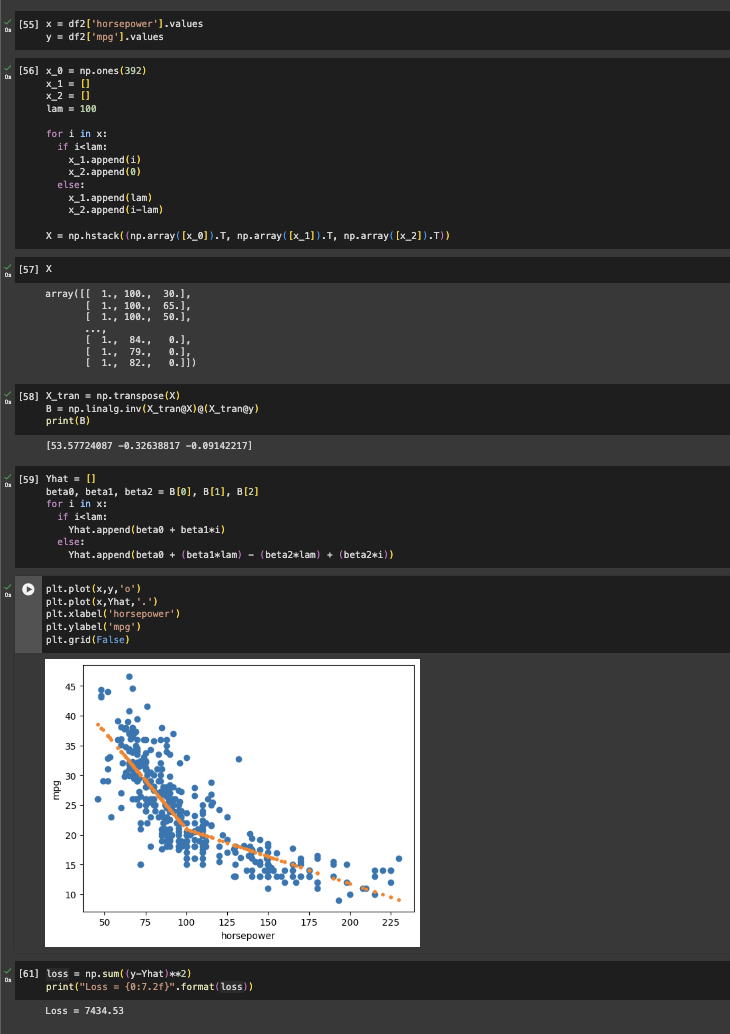
\includegraphics[trim={0 1.9cm 0 0},clip]{Screenshot 2024-02-15 at 19.28.37.png} \\

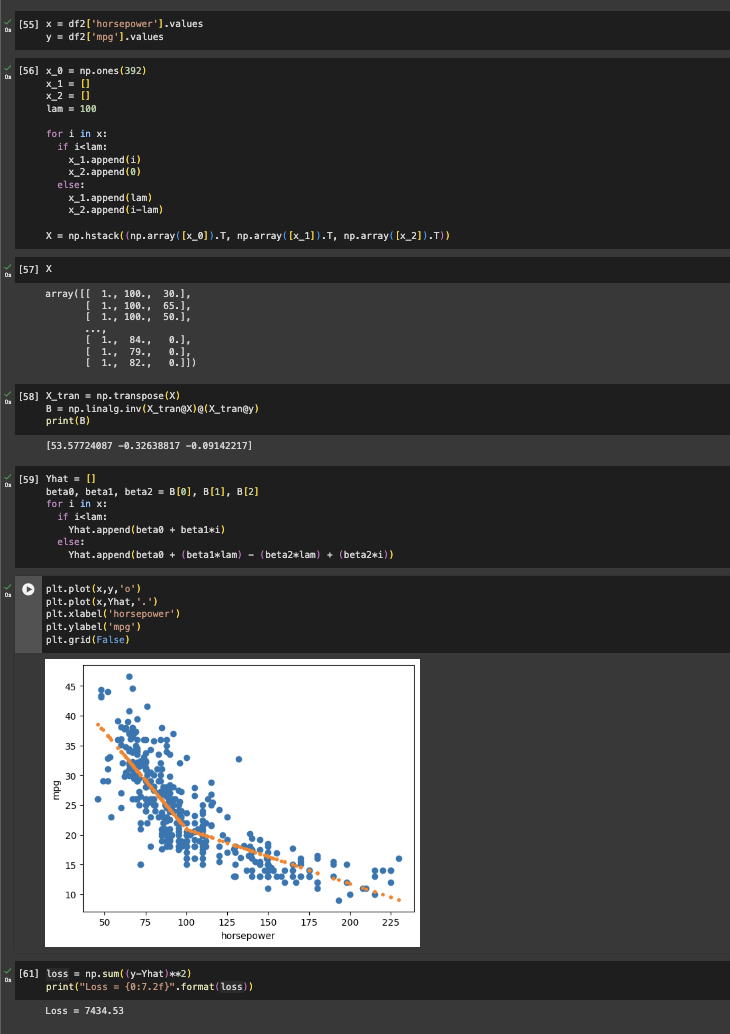
\includegraphics[trim={0 0 0 16.8cm},clip]{Screenshot 2024-02-15 at 19.28.37.png} \\

\subsubsection*{Solution 5 (c)}
\noindent We will choose a lambda using a logspace of values. Then we will find the $\lambda$ which gives the least loss.
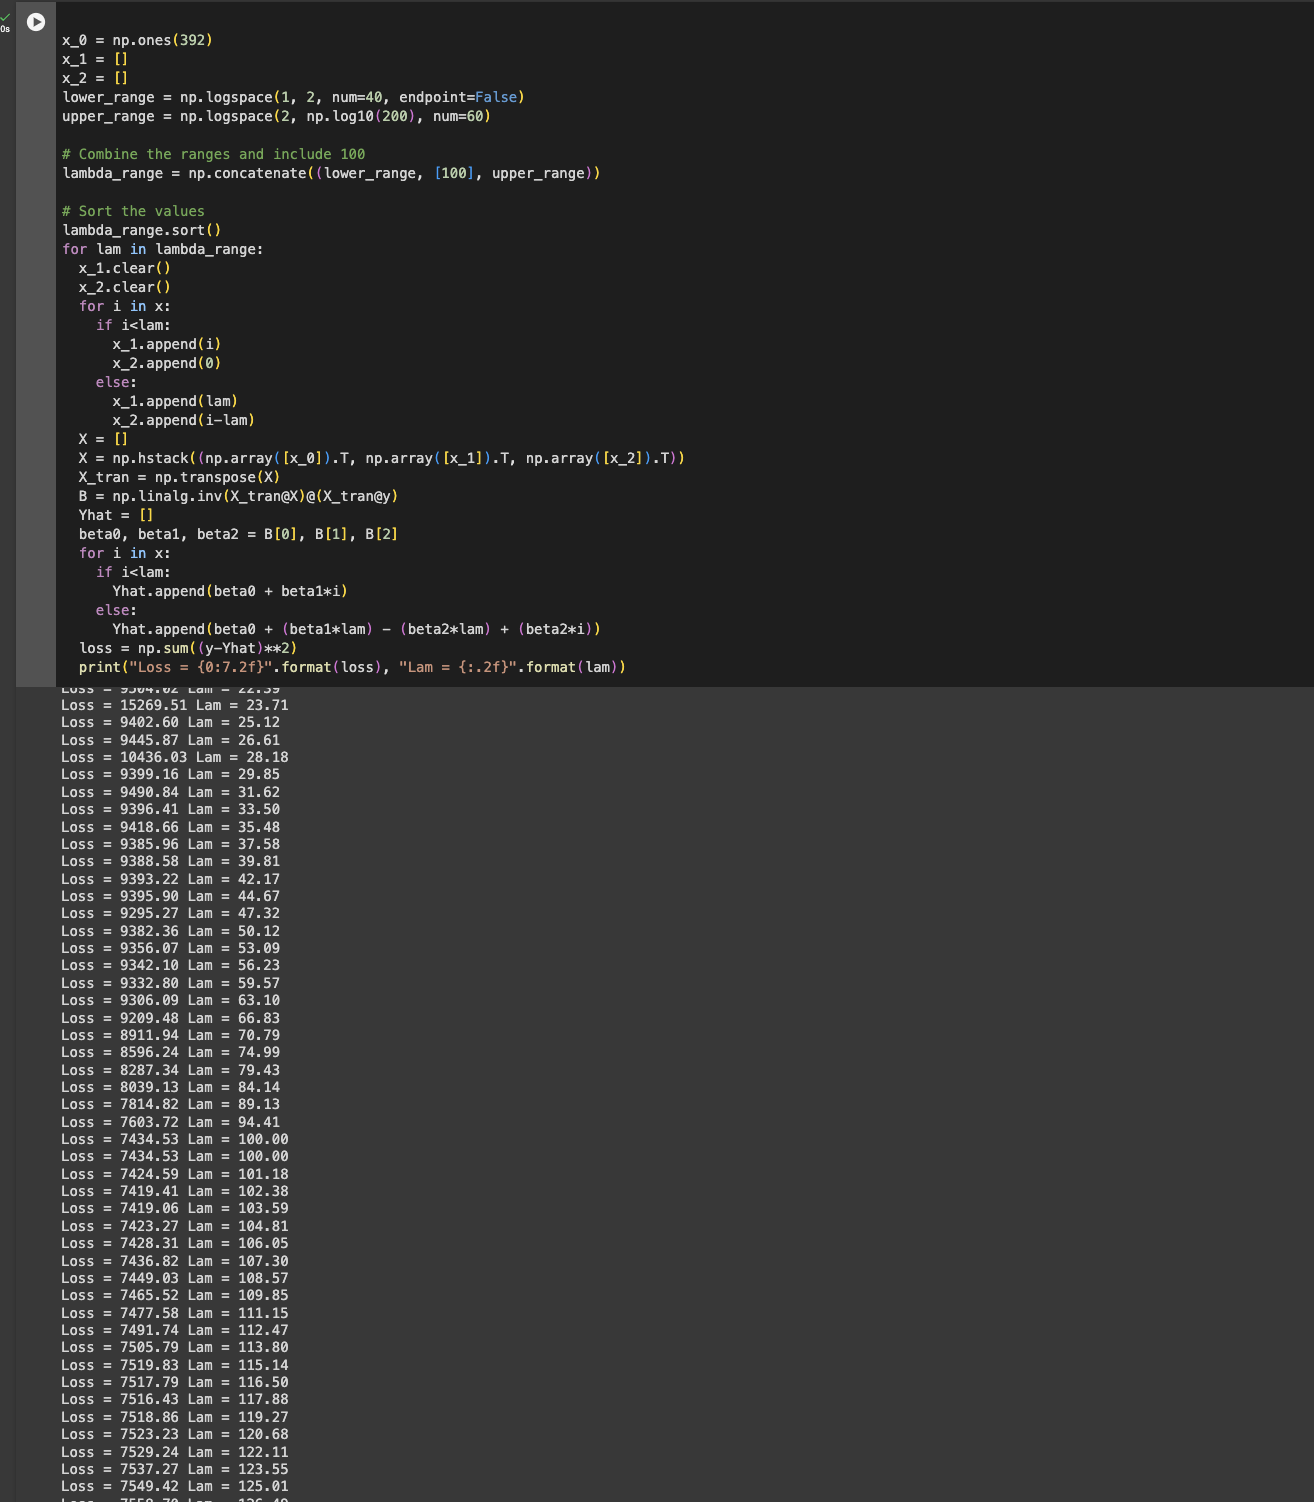
\includegraphics[scale=0.7]{Screenshot 2024-02-15 at 20.37.10.png}
\\ \\ \\ 
The least loss is at the $\lambda$ value 103.59\\ 
We will use this lambda to plot the graph.\\
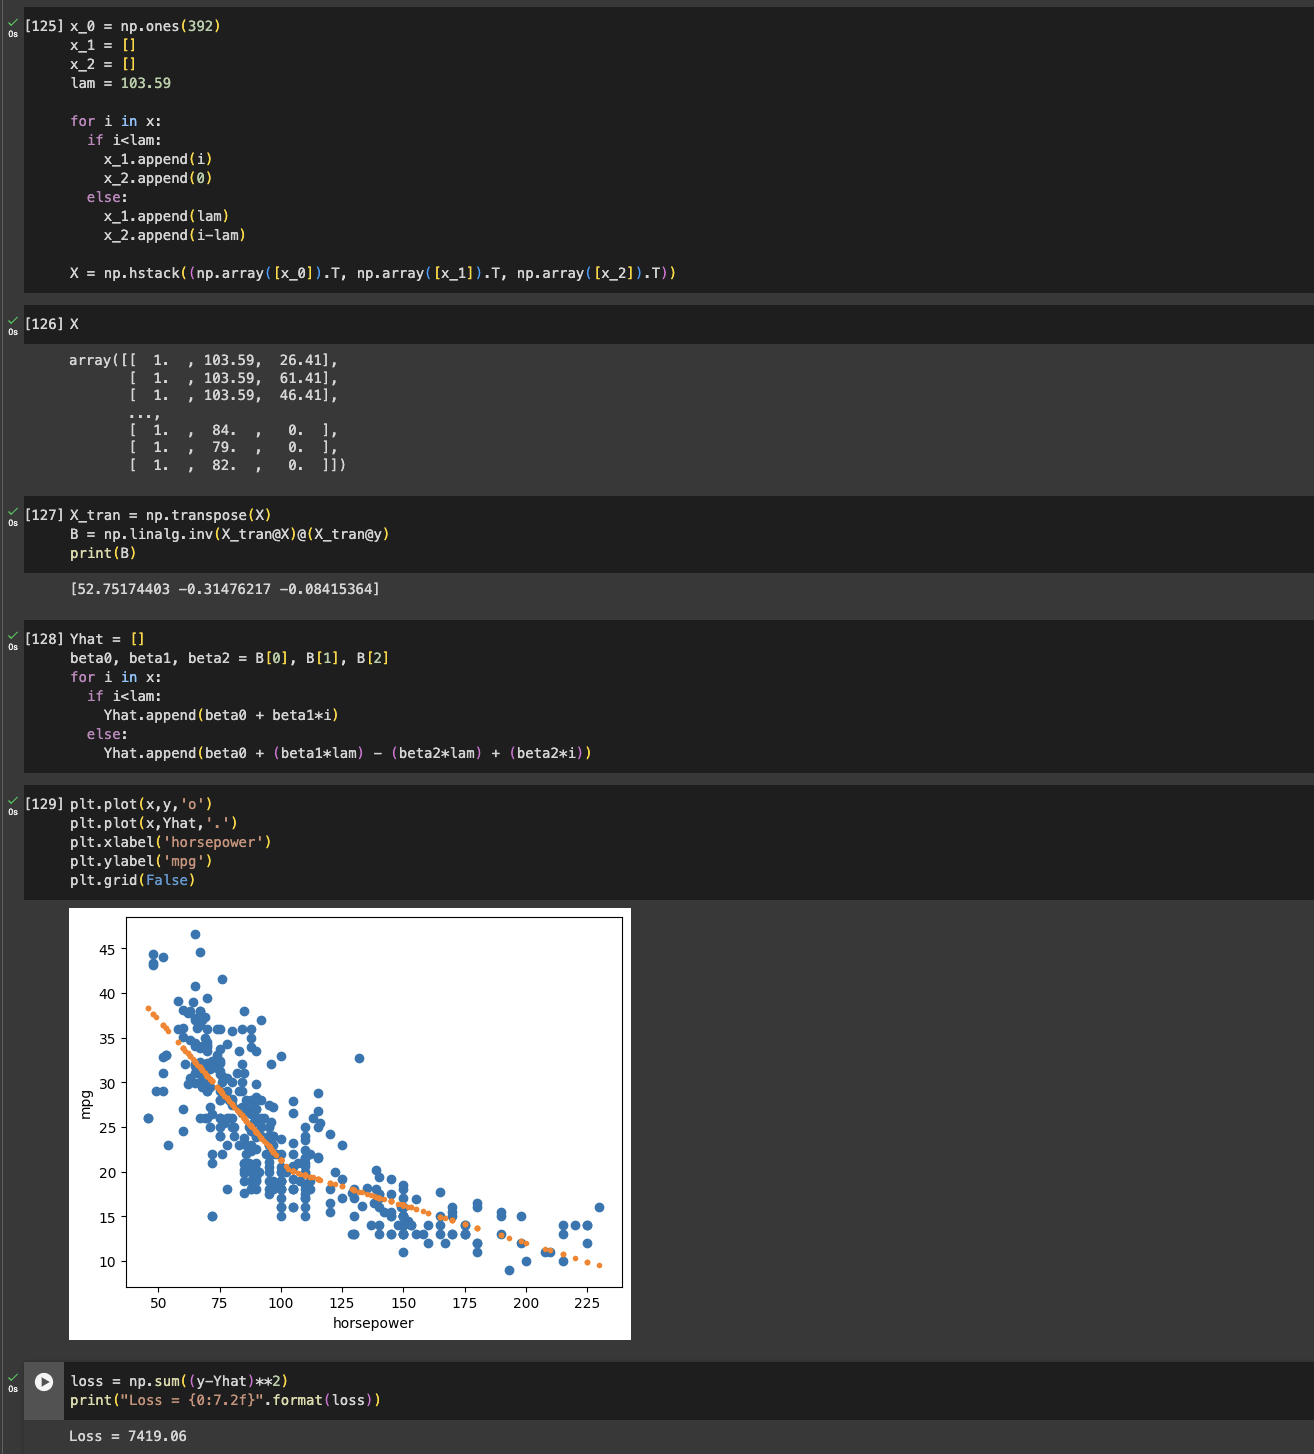
\includegraphics[trim = {0 0 0 13.5cm}, clip,scale = 0.8]{Screenshot 2024-02-15 at 20.40.35.png}
%---------------------------------------------------------------------------------------------
% \begin{problem}

% \section{Segundo Problema}

% \noindent
    
% \end{problem}
%---------------------------------------------------------------------------------------------


\end{document}
